\documentclass[]{article}
\usepackage{amsmath}
\usepackage{amsfonts}
\usepackage{amssymb}
\usepackage{amsthm}
\usepackage{cancel}
\usepackage{graphicx}
\usepackage{pdfpages}
\usepackage{hyperref}

\renewcommand{\thesection}{\arabic{section}}
\renewcommand{\thesubsection}{\thesection.\alph{subsection}}
\renewcommand{\thesubsubsection}{\thesubsection.\roman{subsubsection}}

%opening
\title{EECS 16A HW02}
\author{Bryan Ngo}
\date{2019-09-09}

\begin{document}

\maketitle

\section{Gaussian Elimination}

\subsection{}

\subsubsection{}

\begin{center}
	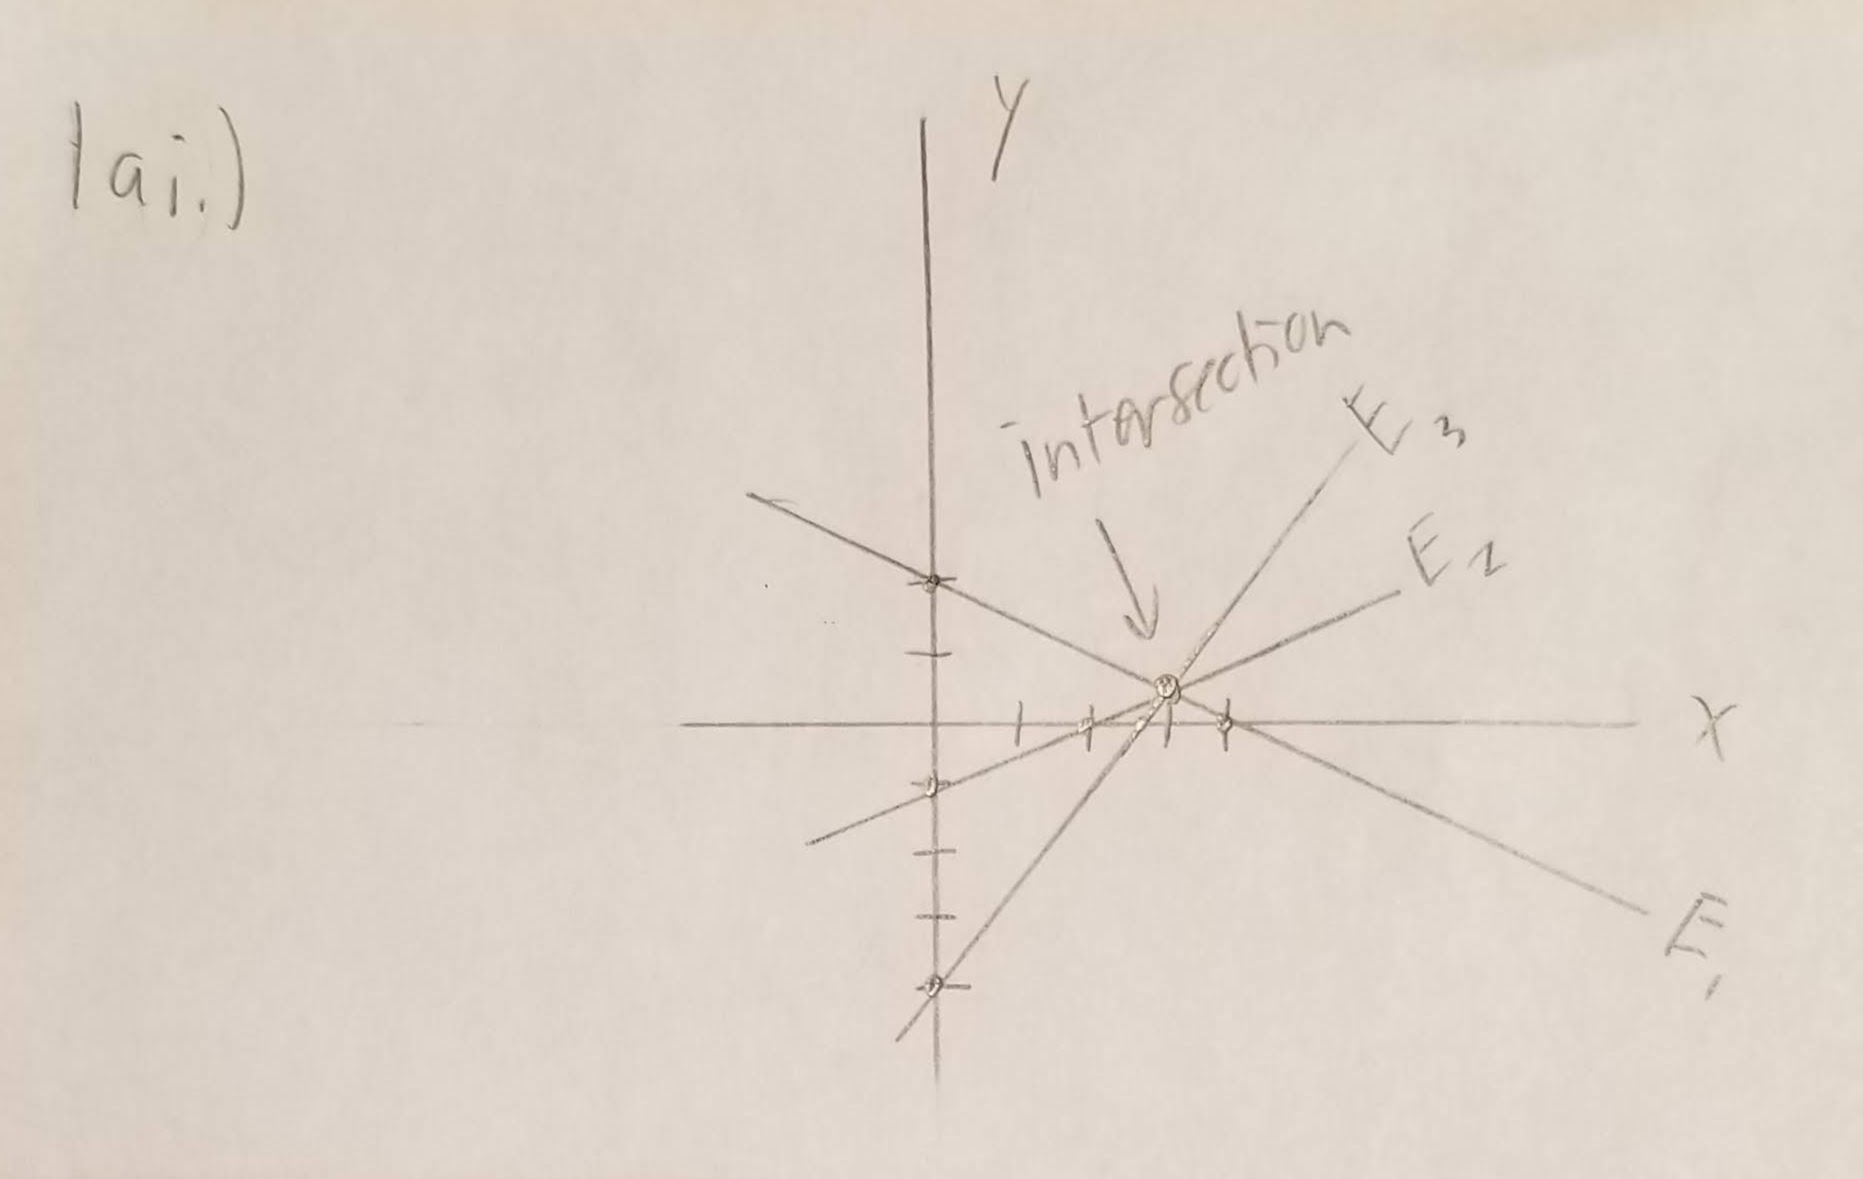
\includegraphics[width=0.7\linewidth]{20190912_160635}
\end{center}

\subsubsection{}

The equation can be written as the augmented matrix
\begin{align}
	&\left[
	\begin{array}{cc|c}
	1 & 2 & 4 \\
	2 & -4 & 4 \\
	3 & -2 & 8
	\end{array}
	\right] \\
	&\Rightarrow \left[
	\begin{array}{cc|c}
	1 & 2 & 4 \\
	0 & -8 & -4 \\
	3 & -2 & 8
	\end{array}
	\right] \quad r_2 - 2r_1 \to r_2 \\
	&\Rightarrow \left[
	\begin{array}{cc|c}
	1 & 2 & 4 \\
	0 & 1 & \frac{1}{2} \\
	3 & -2 & 8
	\end{array}
	\right] \quad r_2 / 2 \to r_2
\end{align}

\begin{center}
	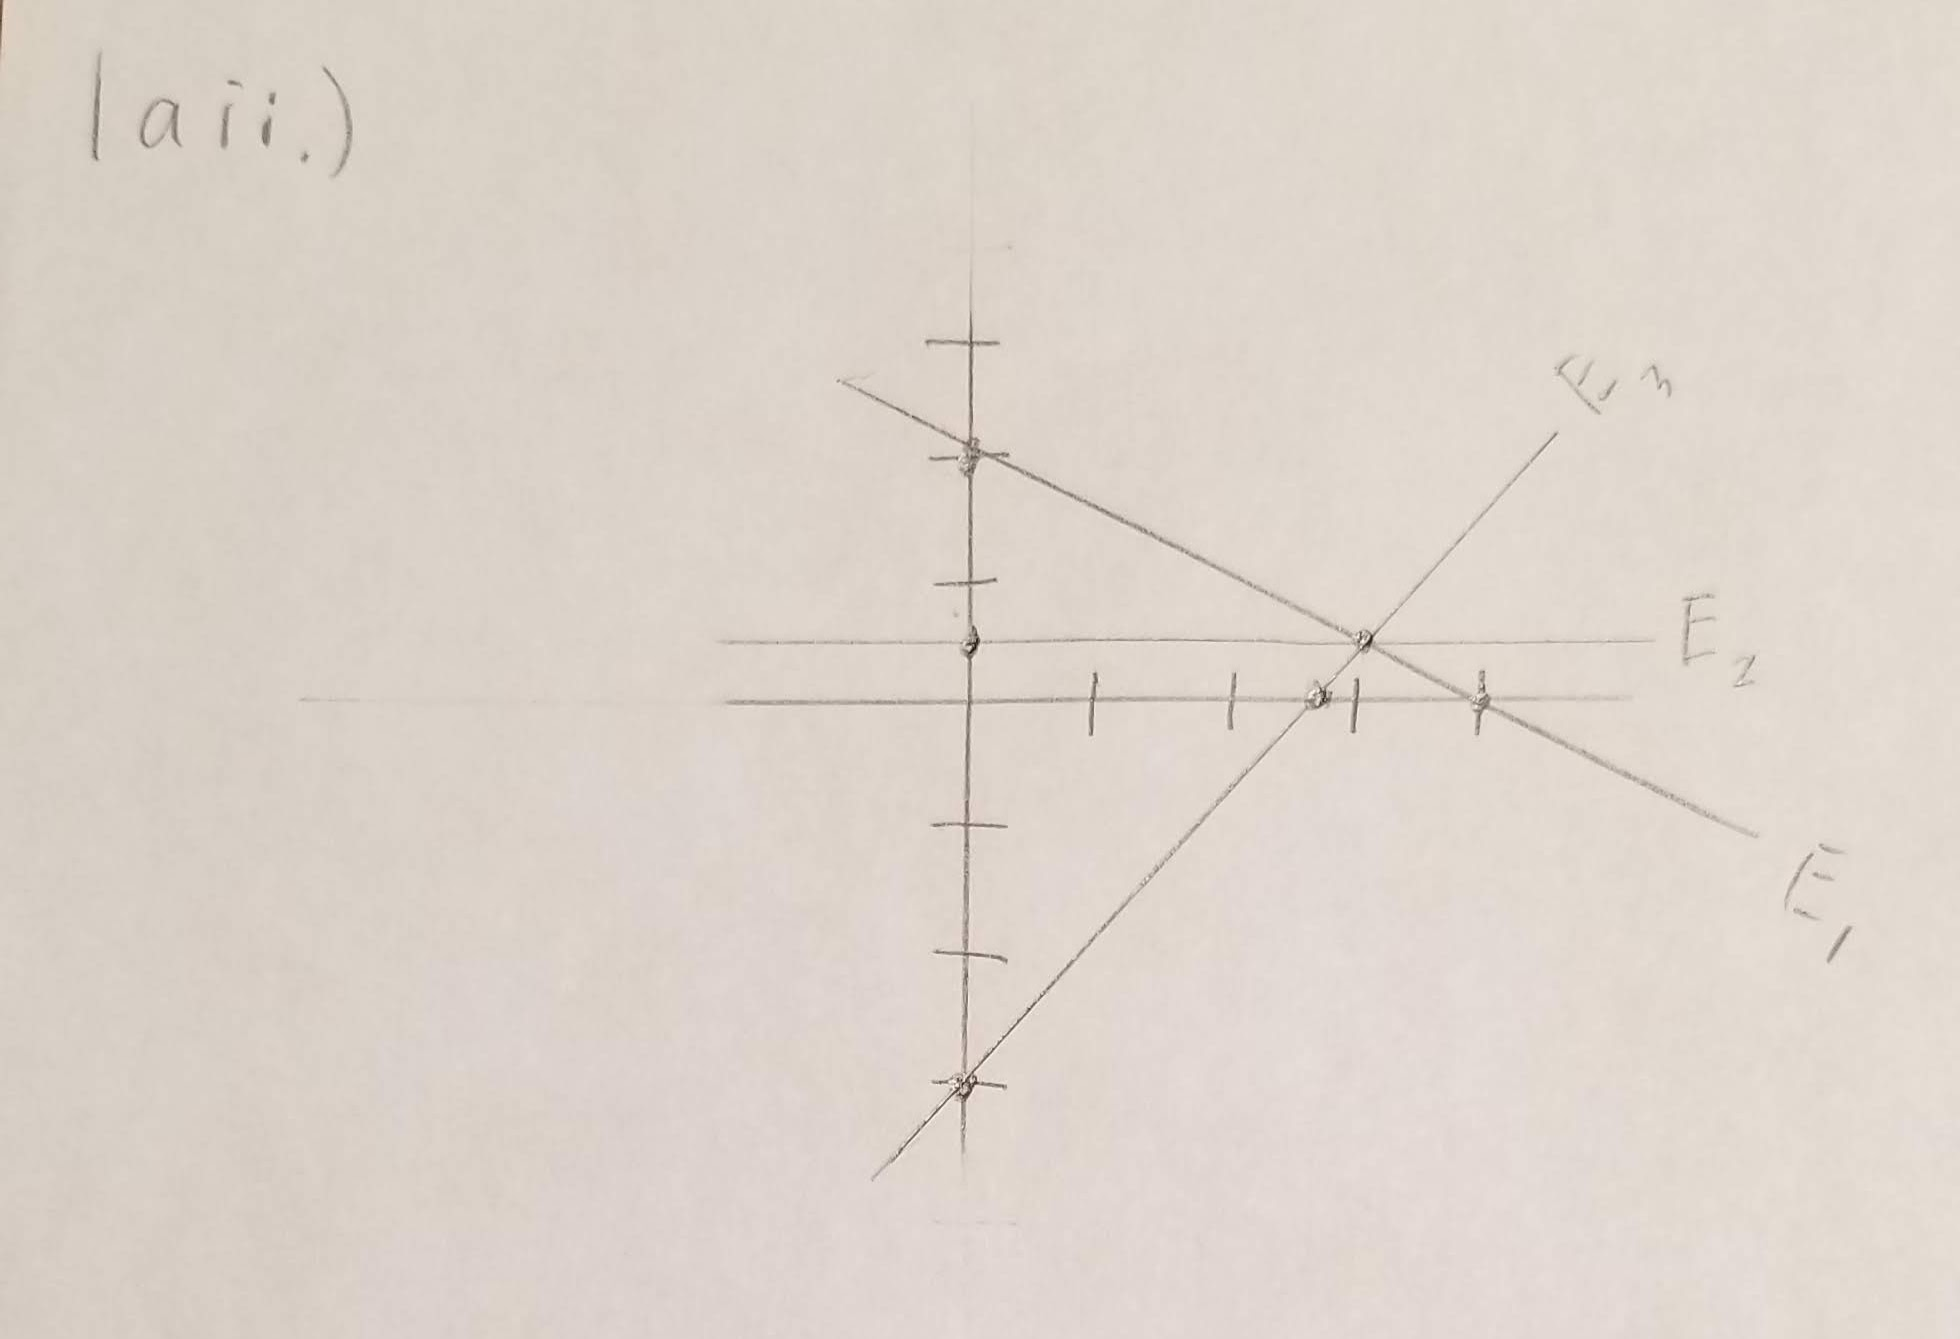
\includegraphics[width=0.7\linewidth]{20190912_160638}
\end{center}

\subsubsection{}

\begin{align}
	&\left[
	\begin{array}{cc|c}
	1 & 2 & 4 \\
	0 & 1 & \frac{1}{2} \\
	4 & 0 & 12
	\end{array}
	\right] \quad r_3 + r_1 \to r_3 \\
	&\Rightarrow \left[
	\begin{array}{cc|c}
	1 & 2 & 4 \\
	0 & 1 & \frac{1}{2} \\
	1 & 0 & 3
	\end{array}
	\right]  \quad r_3 / 4 \to r_3 \\
	&\Rightarrow \left[
	\begin{array}{cc|c}
	1 & 2 & 4 \\
	1 & 0 & 3 \\
	0 & 1 & \frac{1}{2}
	\end{array}
	\right] \quad r_2 \longleftrightarrow r_3
\end{align}
When we graph the system, we notice that \(E_1\) is redundant because it already intersects with \(E_{2,3}\). Specifically, the \emph{unique} solution to the system is \((3, \frac{1}{2})\). \\

\begin{center}
	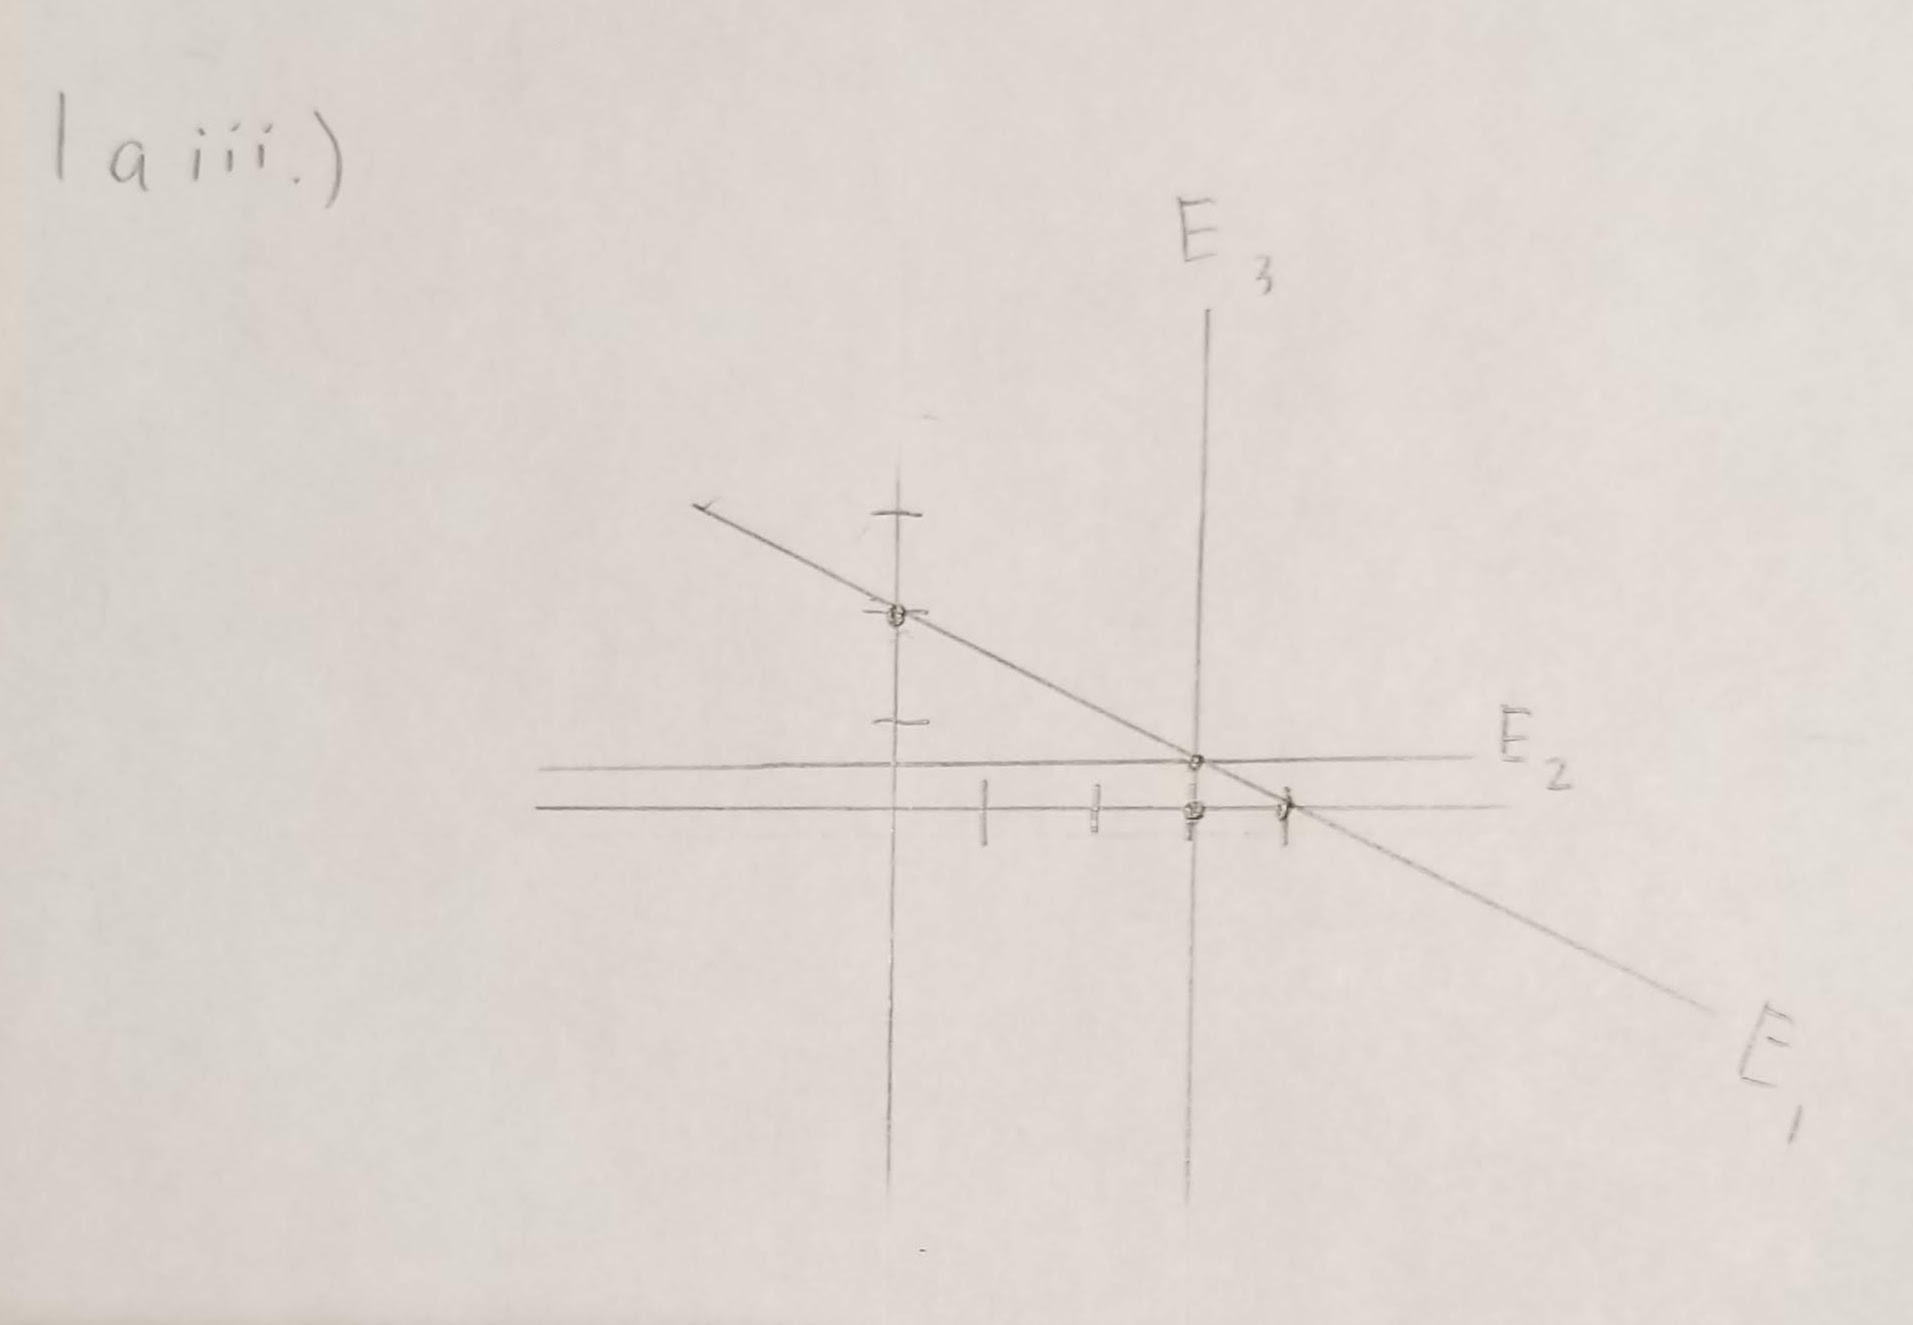
\includegraphics[width=0.7\linewidth]{20190912_160642}
\end{center}

\subsection{}

The given system can be written as the augmented matrix
\begin{align}
	&\left[
	\begin{array}{ccc|c}
	1 & 2 & 5 & 3 \\
	1 & 12 & 6 & 1 \\
	0 & 2 & 1 & 4 \\
	3 & 16 & 16 & 7
	\end{array}
	\right] \\
	&\Rightarrow \left[
	\begin{array}{ccc|c}
	1 & 2 & 5 & 3 \\
	0 & 10 & 1 & -2 \\
	0 & 2 & 1 & 4 \\
	3 & 16 & 16 & 7
	\end{array}
	\right] \quad r_2 - r_1 \to r_2 \\
	&\Rightarrow \left[
	\begin{array}{ccc|c}
	1 & 2 & 5 & 3 \\
	0 & 10 & 1 & -2 \\
	0 & 0 & \frac{4}{5} & \frac{22}{5} \\
	3 & 16 & 16 & 7
	\end{array}
	\right] \quad r_3 - r_2/5 \to r_3 \\
	&\Rightarrow \left[
	\begin{array}{ccc|c}
	1 & 2 & 5 & 3 \\
	0 & 10 & 1 & -2 \\
	0 & 0 & 1 & \frac{11}{2} \\
	3 & 16 & 16 & 7
	\end{array}
	\right] \quad \frac{5}{4}r_3 \to r_3 \\	
	&\Rightarrow \left[
	\begin{array}{ccc|c}
	1 & 2 & 5 & 3 \\
	0 & 10 & 0 & \frac{-15}{2} \\
	0 & 0 & 1 & \frac{11}{2} \\
	3 & 16 & 16 & 7
	\end{array}
	\right] \quad r_2 - r_3 \to r_2 \\
	&\Rightarrow \left[
	\begin{array}{ccc|c}
	1 & 2 & 5 & 3 \\
	0 & 1 & 0 & \frac{-3}{4} \\
	0 & 0 & 1 & \frac{11}{2} \\
	3 & 16 & 16 & 7
	\end{array}
	\right] \quad r_2/10 \to r_2 \\
	&\Rightarrow \left[
	\begin{array}{ccc|c}
	1 & 0 & 5 & \frac{15}{4} \\
	0 & 1 & 0 & \frac{-3}{4} \\
	0 & 0 & 1 & \frac{11}{2} \\
	3 & 16 & 16 & 7
	\end{array}
	\right] \quad r_1 - 2r_2 \to r_1 \\
	&\Rightarrow \left[
	\begin{array}{ccc|c}
	1 & 0 & 0 & -23 \\
	0 & 1 & 0 & \frac{-3}{4} \\
	0 & 0 & 1 & \frac{11}{2} \\
	3 & 16 & 16 & 7
	\end{array}
	\right] \quad r_1 - 5r_3 \to r_1
\end{align}
If we plug in \((-23, -\frac{3}{4}, \frac{11}{2})\), we can see that it satisfies \(E_4\):
\begin{equation}
	3(-23) + 16\left(-\frac{3}{4}\right) + 16 \left(\frac{11}{2}\right) = -69 - 12 + 88 = 7
\end{equation}
which yields our \emph{unique} solution. 

\subsection{}

\begin{proof}
Given our system
\begin{alignat}{6}
	x && + && 2y && + && 5z && = 6 \\
	3x && + && 9y && + && 6z && = 3
\end{alignat}
we can rewrite our system as a matrix-vector product
\begin{equation}\label{eq:1c-matrix-vector}
	\begin{bmatrix}
	1 & 2 & 5 \\
	3 & 9 & 6 
	\end{bmatrix}
	\begin{bmatrix}
	x \\
	y \\
	z
	\end{bmatrix}
	=
	\begin{bmatrix}
	6 \\
	3
	\end{bmatrix}
\end{equation}
Turning our attention to our set \(S\), where
\begin{equation}
	S = 
	\left\lbrace
	\begin{array}{c|c}
	\mathbf{v} & \mathbf{v} = 
	\begin{bmatrix}
	16 \\
	-5 \\
	0
	\end{bmatrix}
	+
	\begin{bmatrix}
	-11 \\
	3 \\
	1
	\end{bmatrix}t, \ t \in \mathbb{R}
	\end{array}
	\right\rbrace
\end{equation}
we can reduce the definition of \(S\) to a single matrix since both matrices in its definition are in \(\mathbb{R}^3\) and \(t \in \mathbb{R}\). This yields us
\begin{equation}
	S = 
	\left\lbrace
	\begin{array}{c|c}
	\mathbf{v} & \mathbf{v} = 
	\begin{bmatrix}
	16 - 11t \\
	-5 + 3t \\
	t
	\end{bmatrix}, \ t \in \mathbb{R}
	\end{array}
	\right\rbrace
\end{equation}
Note that the only thing differentiating elements of \(S\) is the value of \(t\). Referring back to \autoref{eq:1c-matrix-vector}, if we consider our equation in the form \(\mathbf{Av} = \mathbf{b}\), where 
\begin{equation}
	\mathbf{v} = \begin{bmatrix}
	x \\
	y \\
	z
	\end{bmatrix}
\end{equation}
all we have to do is substitute our definition of \(v\) into \autoref{eq:1c-matrix-vector}:
\begin{equation}
	\begin{bmatrix}
	1 & 2 & 5 \\
	3 & 9 & 6 
	\end{bmatrix}
	\begin{bmatrix}
	16 - 11t \\
	-5 + 3t \\
	t
	\end{bmatrix}
	=
	\begin{bmatrix}
	6 \\
	3
	\end{bmatrix}
\end{equation}
Carrying out the matrix multiplication, 
\begin{align}
	\begin{bmatrix}
	(16 - 11t) + 2(-5 + 3t) + 5(t) \\
	3(16 - 11t) + 9(-5 + 3t) + 6(t)
	\end{bmatrix}
	&=
	\begin{bmatrix}
	6 \\
	3
	\end{bmatrix} \\
	\begin{bmatrix}
	16 - \cancel{11t} - 10 + \cancel{6t} + \cancel{5t} \\
	48 - \cancel{33t} - 45 + \cancel{27t} + \cancel{6t}
	\end{bmatrix}
	&=
	\begin{bmatrix}
	6 \\
	3
	\end{bmatrix} \\
	\begin{bmatrix}
	6 \\
	3
	\end{bmatrix}
	&=
	\begin{bmatrix}
	6 \\
	3
	\end{bmatrix}
\end{align}
Thus, we have proved that no matter what value of \(t\), and therefore any element of \(S\) since \(t\) is the only free variable, they will always cancel and you will get a solution to the system, since the resulting calculation satisfies the resultant vector. 
\end{proof}

\subsection{}

Given our rref'ed matrix
\begin{equation}
	\left[
	\begin{array}{ccccc|c}
	1 & 1 & 0 & 0 & 3 & 16 \\
	0 & 0 & 1 & 0 & -3 & -17 \\
	0 & 0 & 0 & 1 & 1 & 5
	\end{array}
	\right]
\end{equation}
A \emph{free variable} is one that is not a pivot. This means that there are 2 free variables in the system, that in the 2nd column and that in the last column. The matrix can be reconverted into a system of equations into 
\begin{alignat}{11}
	x && + && y && && && && && + && 3v && = && 16 \\
	&& && && && z && && && - && 3v && = && -17 \\ 
	&& && && && && && w && + && v && = && 5
\end{alignat}
for which our free variables are \(y, v\) and our pivots are \(x, z, w\). In order to generate the infinite set of solutions, we must solve for the pivots in terms of the free variables. Using simple algebra, we can do this:
\begin{align}
	x(t) &= 16 - y - 3v \\
	z(t) &= 3v + 17 \\
	w(t) &= 5 - v
\end{align}

\section{Boser's Optimal Boba}

\subsection{}

We can represent the single rating as a linear combination of the pure teas weighted by their relative composition in the teas, leading to the system of equations
\begin{alignat}{9}
	\frac{1}{3} \beta && + && \frac{1}{3} \Omega && + && 0 \gamma && + && \frac{1}{3} \epsilon && = && 7 \\
	\frac{1}{3} \beta && + && \frac{1}{3} \Omega && + && \frac{1}{3} \gamma && + && 0 \epsilon && = && 7 \\
	0 \beta && + && \frac{2}{5} \Omega && + && \frac{3}{5} \gamma && + && 0 \epsilon && = && \frac{37}{5} \\
	\frac{2}{3} \beta && + && \frac{1}{3} \Omega && + && 0 \gamma && + && 0 \epsilon && = && \frac{19}{3}
\end{alignat}
for \(\beta\)lack, \(\Omega\)olong, \(\gamma\)reen, and \(\epsilon\)arl Grey tea ratings. This looks like the following matrix-vector multiplication and augmented matrix:
\begin{gather}
	\begin{bmatrix}
	\frac{1}{3} & \frac{1}{3} & 0 & \frac{1}{3} \\
	\frac{1}{3} & \frac{1}{3} & \frac{1}{3} & 0 \\
	0 & \frac{2}{5} & \frac{3}{5} & 0 \\
	\frac{2}{3} & \frac{1}{3} & 0 & 0
	\end{bmatrix}
	\begin{bmatrix}
	\beta \\
	\Omega \\
	\gamma \\
	\epsilon
	\end{bmatrix}
	=
	\begin{bmatrix}
	7 \\
	7 \\
	\frac{37}{5} \\
	\frac{19}{3}
	\end{bmatrix} \\
	\left[
	\begin{array}{cccc|c}
	\frac{1}{3} & \frac{1}{3} & 0 & \frac{1}{3} & 7 \\
	\frac{1}{3} & \frac{1}{3} & \frac{1}{3} & 0 & 7 \\
	0 & \frac{2}{5} & \frac{3}{5} & 0 & \frac{37}{5} \\
	\frac{2}{3} & \frac{1}{3} & 0 & 0 & \frac{19}{3}
	\end{array}
	\right]
\end{gather}
Given the complexity of this system, we employ a faster means of solving the system, yielding Prof. Ranade's ratings for the pure teas: 
\begin{equation}
	\left[
	\begin{array}{cccc|c}
	1 & 0 & 0 & 0 & 7 \\
	0 & 1 & 0 & 0 & 5 \\
	0 & 0 & 1 & 0 & 9 \\
	0 & 0 & 0 & 1 & 9
	\end{array}
	\right]
\end{equation}
or \(7 = \beta\)lack, \(5 = \Omega\)olong, \(9 = \gamma\)reen, and \(9 = \epsilon\)arl Grey. 

\subsection{}

Prof. Ranade's optimal tea can be created using her ratings for the pure teas by the following linear equation
\begin{equation}
	7a + 5b + 9c + 9d = S
\end{equation}
where pure tea proportions \(a + b + c + d = 1\) and \(S\) is the final score. It can be easily shown that it is impossible to get \(S > 9\) from Prof. Ranade within the constraints of the problem because having any weight other than 0 in any non-9 term would bring the score below 9. Thus, a combination that would maximize Ranade's score could be any proportion of Oolong and Earl Grey tea, e.g. \(\frac{28}{53}\) Oolong tea and \(\frac{25}{53}\) Earl Grey. 

\section{Finding Charges from Potential Measurements}

Assuming we ignore \(k\) for the purposes of calculation (since it cancels out), we can simply substitute the potentials \(U_{1,2,3}\) into the formulas for the linear combination of the charges, 
\begin{align}
	\frac{Q_1}{\sqrt{2}} + \frac{Q_2}{\sqrt{5}} + \frac{Q_3}{2} &= \frac{4 + 3\sqrt{5} + \sqrt{10}}{2 \sqrt{5}} \\
	Q_1 + \frac{Q_2}{\sqrt{2}} + Q_3 &= \frac{2 + 4 \sqrt{2}}{\sqrt{2}} \\
	\frac{Q_1}{2} + \frac{Q_2}{\sqrt{5}} + \frac{Q_3}{\sqrt{2}} &= \frac{4 + \sqrt{5} + 3\sqrt{10}}{2 \sqrt{5}}
\end{align}
Converting into a matrix-vector multiplication, 
\begin{equation}
	\begin{bmatrix}
	\frac{1}{\sqrt{2}} & \frac{1}{\sqrt{5}} & \frac{1}{2} \\
	1 & \frac{1}{\sqrt{2}} & 1 \\
	\frac{1}{2} & \frac{1}{\sqrt{5}} & \frac{1}{\sqrt{2}}
	\end{bmatrix}
	\begin{bmatrix}
	Q_1 \\
	Q_2 \\
	Q_3
	\end{bmatrix}
	=
	\begin{bmatrix}
	\frac{4 + 3\sqrt{5} + \sqrt{10}}{2 \sqrt{5}} \\
	\frac{2 + 4 \sqrt{2}}{\sqrt{2}} \\
	\frac{4 + \sqrt{5} + 3\sqrt{10}}{2 \sqrt{5}}
	\end{bmatrix}
\end{equation}

See the iPython pages for the charge calculations, where we get 
\begin{align}
	Q_1 &= 1 \\
	Q_2 &= 2 \\
	Q_3 &= 3
\end{align}

\section{Kinematic Model for a Simple Car}

\subsection{}

\begin{center}
	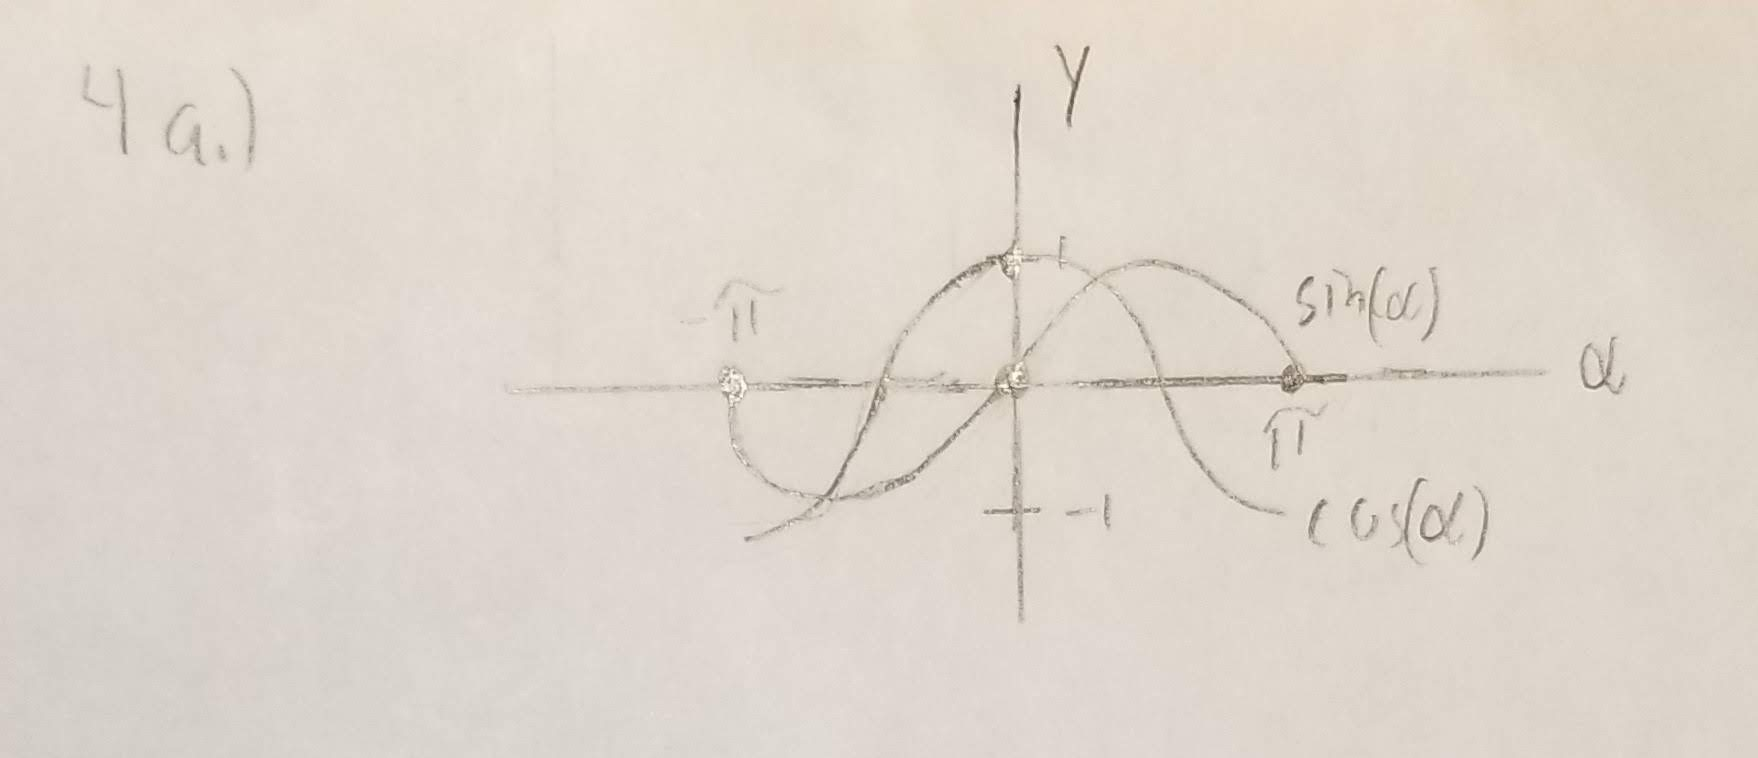
\includegraphics[width=0.7\linewidth]{20190913_220943}
\end{center}

We can justify the small-angle approximations
\begin{align}
	\sin(\alpha) \approx 0 \\
	\cos(\alpha) \approx 1
\end{align}
for some \(\alpha \approx 0\) because, as the graphs of the sine and cosine functions clearly indicate, they get very close to those approximate values around \(\alpha = 0\). 

\subsection{}

See the iPython pages for 5.b-d. \\
\\
First we simplify the \emph{nonlinear} system of equations
\begin{align}
	x[k + 1] &= x[k] + v[k] \cos(\theta[k]) \Delta t \\
	y[k + 1] &= y[k] + v[k] \sin(\theta[k]) \Delta t \\
	\theta[k + 1] &= \theta[k] + \frac{v[k]}{L} \tan(\phi[k]) \Delta t \\ \label{eq:4b-turning-angle}
	v[k + 1] &= v[k] + a[k] \Delta t
\end{align}
Substituting our small angle approximations,
\begin{align}
	x[k + 1] &= x[k] + v[k]\Delta t \\
	y[k + 1] &= y[k] \\
	\theta[k + 1] &= \theta[k] \\
	v[k + 1] &= v[k] + a[k] \Delta t
\end{align}
Splitting up the system into 2 vectors, 
\begin{align}
	\begin{bmatrix}
	x[k + 1] \\
	y[k + 1] \\
	\theta[k + 1] \\
	v[k + 1]
	\end{bmatrix}
	&=
	\begin{bmatrix}
	x[k] + 0.1v[k] \\
	y[k] \\
	\theta[k] \\
	v[k]
	\end{bmatrix}
	+
	\begin{bmatrix}
	0 \\
	0 \\
	0 \\
	0.1 a[k]
	\end{bmatrix} \\
	\begin{bmatrix}
	x[k + 1] \\
	y[k + 1] \\
	\theta[k + 1] \\
	v[k + 1]
	\end{bmatrix}
	&=
	\begin{bmatrix}
	1 & 0 & 0 & 0.1 \\
	0 & 1 & 0 & 0 \\
	0 & 0 & 1 & 0 \\
	0 & 0 & 0 & 1
	\end{bmatrix}
	\begin{bmatrix}
	x[k]\\
	y[k] \\
	\theta[k] \\
	v[k]
	\end{bmatrix}
	+
	\begin{bmatrix}
	0 \\
	0 \\
	0 \\
	0.1 a[k]
	\end{bmatrix} \\
	\begin{bmatrix}
	x[k + 1] \\
	y[k + 1] \\
	\theta[k + 1] \\
	v[k + 1]
	\end{bmatrix}
	&=
	\underbrace{
	\begin{bmatrix}
	1 & 0 & 0 & 0.1 \\
	0 & 1 & 0 & 0 \\
	0 & 0 & 1 & 0 \\
	0 & 0 & 0 & 1
	\end{bmatrix}}_{\mathbf{A}}
	\begin{bmatrix}
	x[k]\\
	y[k] \\
	\theta[k] \\
	v[k]
	\end{bmatrix}
	+
	\underbrace{\begin{bmatrix}
	0 & 0 \\
	0 & 0 \\
	0 & 0 \\
	0.1 & 0
	\end{bmatrix}}_{\mathbf{B}}
	\begin{bmatrix}
	a[k] \\
	\phi[k]
	\end{bmatrix}
\end{align}

\subsection{}

The motion between the linear and non-linear models are extremely similar in this case. This is probably due to the extremely small turning angle \(\phi\). This means that according to \autoref{eq:4b-turning-angle}, our \(\theta[k + 1]\), regardless of the step interval, is effectively \(0\) and thus the rest of the state vectors do not deviate very much from each other. 

\subsection{}

In this case, the trajectories of the linear and nonlinear state vectors are extremely different. This is because \(0.5 \ \text{rad}\) is a relatively large angle that is non-negligible. This means our small angle approximations have massive errors and deviate heavily from the real path. 

\section{Fountain Codes}

\subsection{}

An example in which \(a\) is unrecoverable but \(b, c\) are is the received vector
\begin{equation}
	\mathbf{r} = 
	\begin{bmatrix}
	\star \\
	b \\
	c \\
	\star \\
	b \\
	c
	\end{bmatrix}
\end{equation}
Since both \(a\) entries are corrupted, we must reject them from the system, making it impossible to recover. 

\subsection{}

Our goal is to find a matrix \(\mathbf{G}_R\) such that
\begin{equation}
	\mathbf{G}_R
	\begin{bmatrix}
	a \\
	b \\
	c
	\end{bmatrix}
	=
	\begin{bmatrix}
	a \\
	b \\
	c \\
	a \\
	b \\
	c
	\end{bmatrix}
\end{equation}
The matrix in question is 
\begin{equation}
	\mathbf{G}_R = 
	\begin{bmatrix}
	1 & 0 & 0 \\
	0 & 1 & 0 \\
	0 & 0 & 1 \\
	1 & 0 & 0 \\
	0 & 1 & 0 \\
	0 & 0 & 1
	\end{bmatrix}
\end{equation}
which is nothing more than 2 \(\mathbf{I}_3\) matrices concatenated vertically. 

\subsection{}

The augmented matrix is
\begin{equation}
	\left[
	\begin{array}{ccc|c}
	1 & 0 & 0 & 7 \\
	0 & 1 & 0 & \star \\
	0 & 0 & 1 & \star \\
	1 & 1 & 0 & 3 \\
	1 & 0 & 1 & 4 \\
	0 & 1 & 1 & \star \\
	1 & 1 & 1 & \star
	\end{array}
	\right]
\end{equation}
Since the corrupted rows are unusable, we can simply ignore them, leaving us with the augmented matrix
\begin{align}
	&\left[
	\begin{array}{ccc|c}
	1 & 0 & 0 & 7 \\
	1 & 1 & 0 & 3 \\
	1 & 0 & 1 & 4
	\end{array}
	\right] \\
	&\Rightarrow \left[
	\begin{array}{ccc|c}
	1 & 0 & 0 & 7 \\
	0 & 1 & 0 & -4 \\
	1 & 0 & 1 & 4
	\end{array}
	\right] \quad r_2 - r_1 \to r_2 \\
	&\Rightarrow \left[
	\begin{array}{ccc|c}
	1 & 0 & 0 & 7 \\
	0 & 1 & 0 & -4 \\
	0 & 0 & 1 & -3
	\end{array}
	\right] \quad r_3 - r_1 \to r_3
\end{align}
leaving us with the original message
\begin{equation}
	\mathbf{m} = 
	\begin{bmatrix}
	7 \\
	-4 \\
	-3
	\end{bmatrix}
\end{equation}

\subsection{}

Bob can recover the message from any 3 \emph{or} 4 symbols he receives using \(\mathbf{G}_F\), given certain constraints. \\
\\
Suppose that 3 symbols are correctly received. This means that 4/7 rows are rejected from \(\mathbf{G}_F\). This leaves us with a system of linear equations with 3 unknowns and 3 equations. There are 3 cases. The system can either have no solutions (geometrically, if the 3 planes do not have a common intersection), or infinite (if one of the planes is a scalar multiple of the other), there exists a set of recoverable solutions for \(\mathbf{r}\). \\
\\
Suppose that 4 symbols are correctly received, leaving 3/7 rows rejected. This leaves us with a system with 3 unknowns and 4 equations. While this does not always guarantee a unique solution (e.g. all the equations could be scalar multiples), it is more likely to have a unique solution than 3 given symbols, since there are more possible constraints on \(\mathbf{r}\). 

\subsection{}

I prefer \(\mathbf{G}_F\) because there is 1 more row than \(\mathbf{G}_R\), so there is more redundancy when transmitting the message. This means \(\mathbf{G}_F\) can handle more corruption. 

\section{Homework Process and Study Group}

I did this homework by myself. 

\newpage

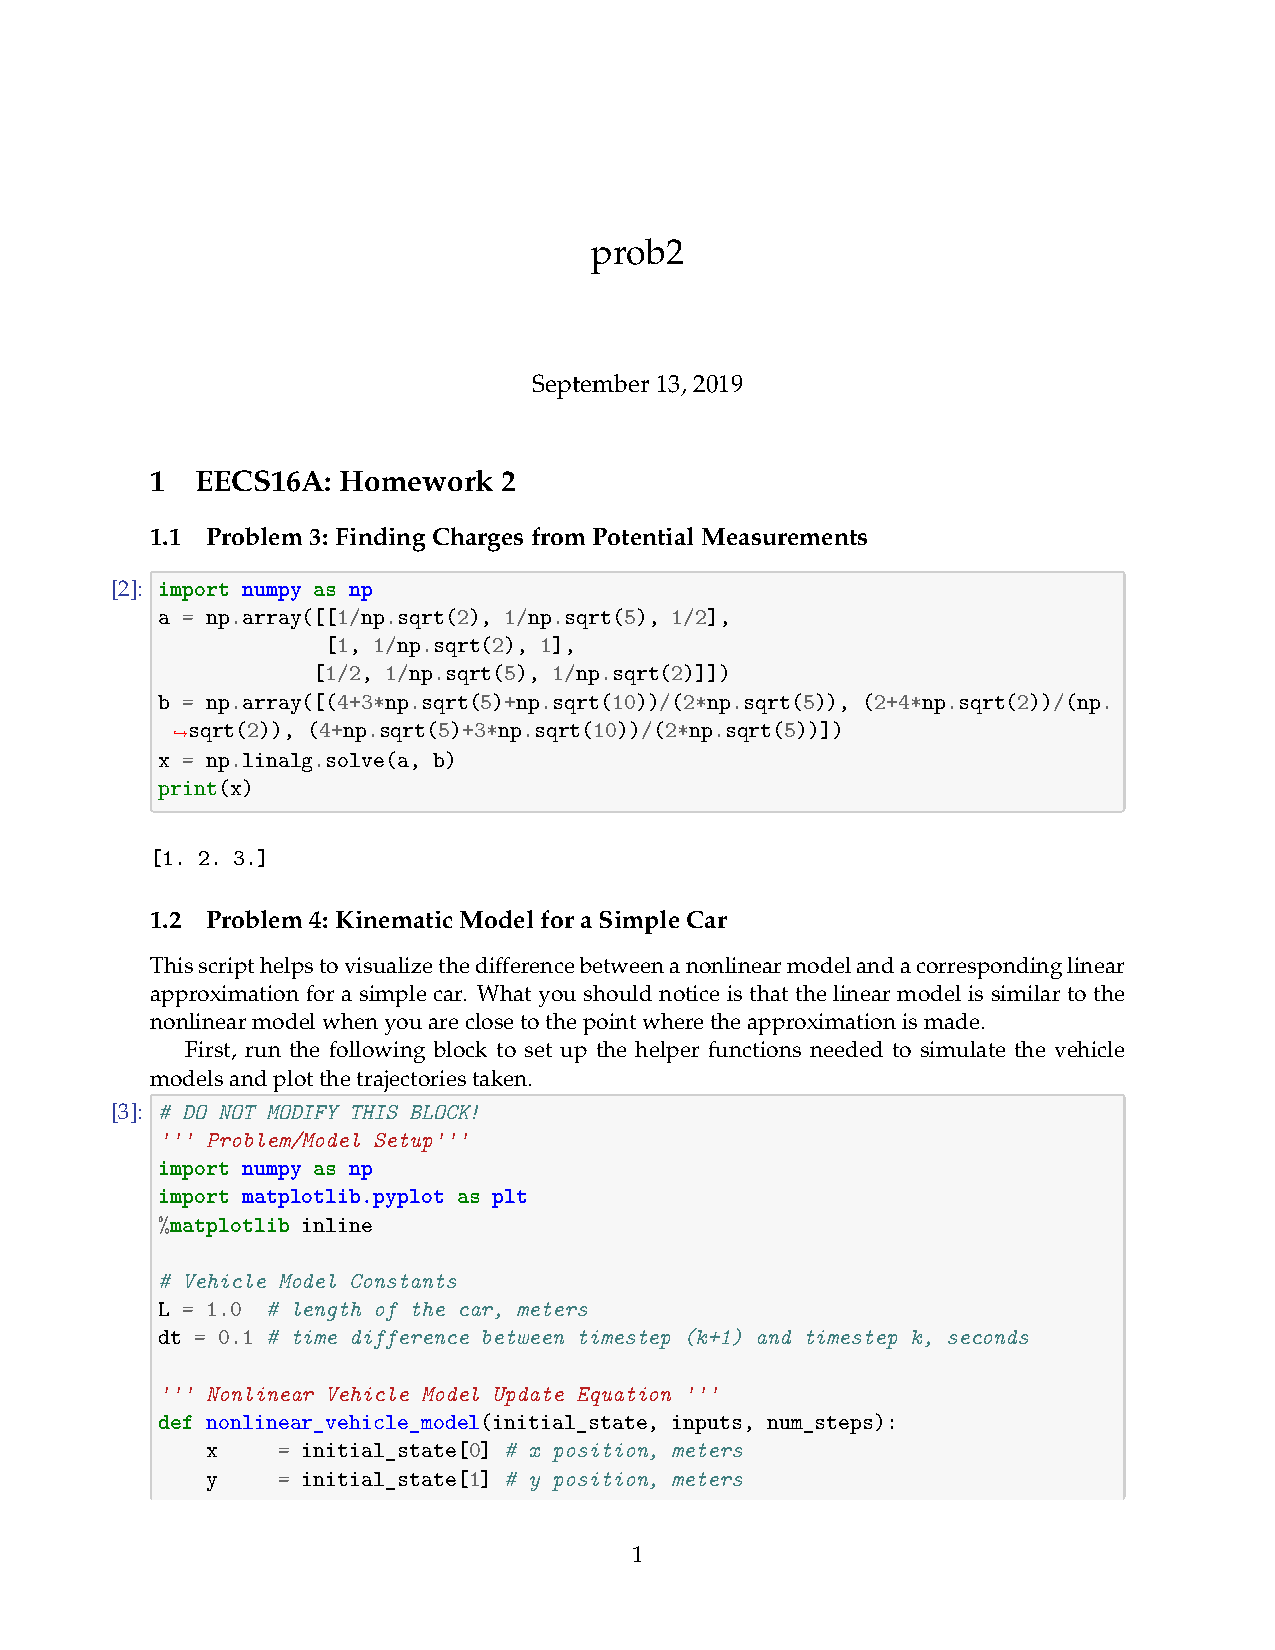
\includepdf[pages=-]{prob2.pdf}

\end{document}